\documentclass[a4paper,10pt]{article}

\usepackage[margin=2cm]{geometry}
\usepackage{graphicx}
\usepackage{amsmath}
\usepackage{array}
\usepackage{hyperref}
\usepackage[all]{hypcap}
\usepackage{listings}
\lstdefinestyle{TerminalStyle}{
  language=bash,
  basicstyle=\small\sffamily,
  numbers=left,
  numberstyle=\tiny,
  numbersep=3pt,
  frame=tb,
  columns=fullflexible,
  linewidth=0.9\linewidth,
  xleftmargin=0.1\linewidth
}
\lstdefinestyle{HtmlStyle}{
  language=html,
  basicstyle=\small\sffamily,
  numbers=left,
  numberstyle=\tiny,
  numbersep=3pt,
  frame=tb,
  columns=fullflexible,
  linewidth=0.9\linewidth,
  xleftmargin=0.1\linewidth
}
\lstdefinestyle{OutputStyle}{
  language=html,
  basicstyle=\small\sffamily,
  frame=tb,
  columns=fullflexible,
  linewidth=0.9\linewidth,
  xleftmargin=0.1\linewidth
}

\setlength{\parindent}{0pt}
\setlength{\parskip}{1ex plus 0.5ex minus 0.2ex}
\title{
\includegraphics[width=12cm]{Eeufeeslogo.jpg} \\
       Department of Computer Science \\
       University of Pretoria \\
       \vspace{0.5cm}
       Software Engineering\\
       COS301 Main Project \\
       \vspace{0.5cm}
       \begin{large} \textbf{Team CodeX}\\ ReRoute Systems\end{large}}

\date{} 
\author{	Bondjobo, Jocelyn 		13232852 		\\
		Malangu, Daniel		13315120		\\
		Kirker, Tim			11152402		\\
		Hammond, Eunice		13222563		\\
		Burgers, Heinrich		15059538		\\
}

\begin{document}
\maketitle
\thispagestyle{empty}
\clearpage

\newpage
\pagenumbering{roman}
\thispagestyle{empty}
\tableofcontents
\clearpage

\newpage
\pagenumbering{arabic}

\section{Introduction}

	\subsection{Background} 
	Reroute Systems is a software company with different in-house developed applications. The Purchase Management System application is the main application and mainly active in the 		pharmaceutical space. The main functionality of the system is routing of request for products from account holders to the various wholesalers / suppliers, receiving the result of the order and route answer back to account holder.
	
	\subsection{Purpose} 	
	For the account holder to request a product he/she must search for it against the database with all the product information, the challenge is that each wholesalers / suppliers can name/describe the product differently and when the account holder do the search against the master product list the same product must be displayed across all wholesalers / suppliers using the link between master product list and the different wholesalers / suppliers product list (the user compare the prices of same product across the wholesalers / suppliers before making a decision)
	\subsection{Scope} 
	The core of the system is a search engine which is enriched with functionality
of performing some machine learning in order to retrieve the product in a master file found in a Databased running on the server through http calls. The high level modules and their responsibilities are shown in the figure below. \\ \\
	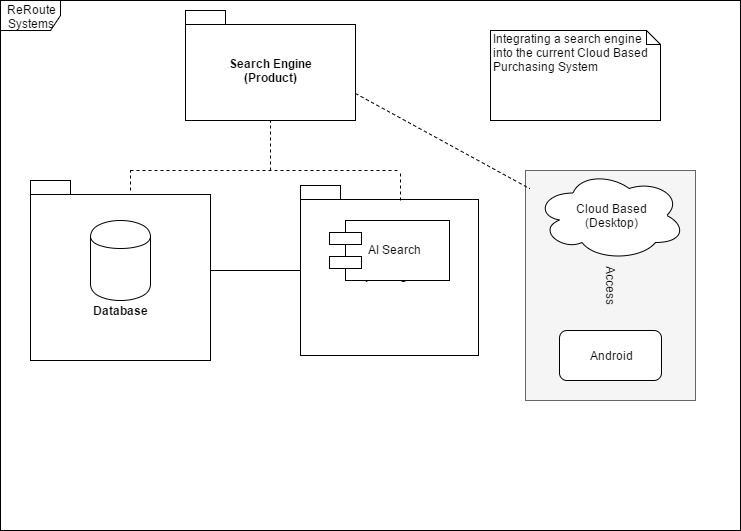
\includegraphics[scale=0.62]{scope1.jpg}
	\subsection{Definitions, Acronyms, and Abbreviations} 

	\begin{itemize} 
	\item Cloud-based : refers to applications, services or resources made available to users on demand via the Internet from a cloud computing provider's servers.
	\item Android : Mobile Operating System that allows the mobile phone to operate and install different apps in it.
	\item AI Search : The use of Artificial Intelligence to serch the database by implementing machine learning techniques and other algorithms to find and retrieve data
	\end{itemize}
	\subsection{References} 
		To be completed 
	\subsection{Overview} 
	The Purchase Management System application is the main application and mainly active in the pharmaceutical space and called \textbf{Smart Rep} that can be found on Google Play store. It allows to place orders of product through mobile devices such as Android and also through Desktop as it is a cloud based system. This system monitors the routing of orders from devices to the server to different wholesalers and bring back the result.

	\newpage

\section{Overall Description}

\subsection{Product Perspective}
        \subsubsection{System Interface}{
			\begin{enumerate} 
				\item User Interface:
					\begin{itemize}
				\item Functionality:\\
					The functionality of the user interface is to allow the user to interact with the system. Through this aspect of the system the user can perform all the functions necessary to use the smart search of the system. Through this the user is able to specify the search criteria to be used by the system.\\
				\item How functionality achieves requirements:\\	
					The user interface allows the functionality of the application to meet the requirements. The user is able to search for any product based on any value they enter int. The user is able to be displayed information of products, that closely based on keywords and values or any thing resembling the name. \\
					\end{itemize}
				\item Hardware Interface:
					\begin{itemize}
					\item Functionality:\\
					The functionality of this system interface is the physical hardware that allows software operation. The hardware in this case is specifically the mobile devices on which the apps run and the computers the websites usually accessed through.\\
				\item How functionality achieves requirements :\\
					This hardware will allow the achievement of the requirements by facilitating the operation of the application. The user will be able to press the physical device screen in order to use the search capabilities and other features of the application. The networking hardware of the components such as the wireless fidelity infrastructure or LAN connections within the devices which will allow for communication to the system server.
				\end{itemize}
				\item Software Interface:
					\begin{itemize}
					\item Functionality:\\
						The functionality of the software interface is to facilitate the communication between the hardware infrastructure of the devices running the application front-end and Reroute Server. An example of this would be the operating system of the device in use. The operating system would allow the application to make use of the networking infrastructure and communicate the necessary information to the application via RESTful calls. This would enable the device to communicate with the server and perform the necessary requests.
\\
					\item How functionality achieves requirements :\\
This would allow the achievement of the requirements as the communication of the application to the system server is vital to the operation of the Smart Search. By allowing communication over WI-Fi the user is able to comunicate to the server from any location  or just stick to older and more familar devices such as computers, fulfilling the requirement .
					\end{itemize}
			\end{enumerate} 
}

		
            \subsubsection{User Interface}
	    {All users will be able use to the Smart Search system from their device when the application is launched.
For the account user interface, the registered userswill be able to login to their account, using their account information.
\\\\
}

\subsubsection{Hardware Interface}
		{
The actual Wi-Fi interface between the mobile device / computer and Wi-Fi will be abstracted by the phone and will be managed by the actual underlying operating system on the phone. On a computer the LAN interface may also be abstracted by the computer and will be managed by the actual underlying operating system on the computer if a wired connection is to be used.}
            \subsubsection{Software Interface}
            to be completed

	    \subsubsection{Communications Interface}
	 \begin{itemize}
	    \item Users using the web will use HTTP/HTTPS protocol.
	    \item REST calls from the differrent platform to the server API.
	    \item Cloud-based server running the database
	    \end{itemize}
            \subsubsection{Memory}
	    {The desktop application will use a minimum amount of space of roughly 300MB.  the size could dramtically increase due to caching and storage of tof data locally. The size will depend solely on caching of a lot of data. \\
Primary memory(RAM) will use 50MB on average, based on how long the application is being used.}
            \subsubsection{Operations}

            	{The user will require a series of usual and special case operations to be fulfilled by the system. The user will use the system in normal case operations that comprise of searching on any of the different properties of a product. On a usual case the user will search for a product based on the name of the product of interest .\\\\
            	The system will provide a user the option to either save there data, such as variations of product names, locally on the device or remotely on the server.}
           \subsubsection{Sit Adaption Requirements}
        to be completed
		\subsection{Product Functions} {The main function of the Smart Search will be to retrieve product iformation based on the values given to the user. The basic functions will include:  }
	\begin{itemize}
  		\item A search based on a specific property of a product such as the name
	\end{itemize}
    	\subsection{User Characteristics}  
		{ 
	
{The general user will use the system to retrive product information. They will need minimal skill in order to utilise the application, including the ability to connect to the Wi-Fi and use . The general user will have restricted usage of the in-app game and certain privileges that require a user profile. They will not require any additional expertise or education to function the application.\\}
    	\subsection{Constraints}   
to be completed
    	\subsection{Assumptions and Dependencies}
to be completed

	\newpage
		
	\section{Specific Requirements}
This section gives a detailed description of the system requirements. It describes all the functional as well as the quality requirements of the system.

	\subsection{External Interface Requirements}

                 \subsubsection{Software Interfaces}
The application will run on the Android operating system, specifically version 4.0. and upwards. It will also run on iOS operating system version 7.3 and above.

	\subsection{Requirements}
	\subsubsection{Functional Requirements} 
	1.	Fuzzy Search:\\\\
	This program must be able to locate and return products that are related to the searched term. It should be able to return the 	same product if various ways of writing the name is used.\\\\
	
	2.	Fast Run-time:\\\\
	Because there are very large amount of data to be searched, it is vital for our program to be very efficient.  Even though this could be a non-functional requirement, it is vital for this program to be as fast and efficient as possible.\\\\
	
	3.	Handle Concurrent Users:\\\\
	This program will be used by many people, in many different fields simultaneously. It is therefore very important for it to be able to handle multiple users at the same time.\\\\
	
	4.	Scalability:\\\\
	Since it is essential for this system to be efficient with large datasets as well as small datasets, scalability will be a functional requirement. The system’s ability to stay efficient with very large sets of data is an essential part to the system.
	
	\subsubsection{Non-Functional Requirements}
	1.	Predictive Typing:\\\\
	Predictive typing is when the program suggests a possible solution as the user is typing. This is often based on previous searches and most common searches. This will help improve the user experience. \\\\

	2.	Return Generic Medicine:\\\\
	In some cases it will be handy if the program suggested the different generic medicine for the medicine you searched for. This could help users find the product they need even if they are unsure of the name.
	
	3.	Robustness:\\\\
	This product should be able to adapt to different users in various fields as well as to different habits, interfaces, environments and needs of users.  
	
	4.	Storing and using search history: 
	Being able to store the search history will increase the user experience, help with predictive typing and improve the programs ability to learn and adapt.
	
	5.	Machine learning:
	Although it is not essential, the ability to learn from users previous interaction and adapt to it will improve the system’s capability and ability greatly. This can be in both large and small scale, from predicting which datasets to load first to creating new links between seemingly unrelated products. 

	\subsubsection{Use Case Prioritization} 
		\begin{enumerate} 
		\item \textbf{Critical} 
			\begin{itemize} 
				\item Login
                 \subsubsection{User Interfaces}
		 
\includegraphics[scale=0.62]{login.png}

				\item Retrieve Wholesalers Accounts 
				\item Search Product 
				
				\textbf{Pre-condition: } The user has to have been logged in successfully.  \\
				\textbf{Post-condition: }  System returns possible matches, or search not found. \\
				\begin{center}
				\begin{tabular}{ |p{8cm}|p{8cm}| }
				 \hline
  				\textbf{Actor:} User & \textbf{System: Purchase Management System Application} Searching Product \\
				 \hline
				 - & 0. TUCBW System displays search bar\\
				 \hline
				  1. User clicks search bar, and enters product name & 2. System retriveies profile information and displays it\\
				 \hline
				 - & 4. System returns and displays all matches found (name variants inclusive) as well as  generics for product name, arranged according to prices and suppliers. \\
				 \hline
				5. User selects appropriate match, or changes search conditions & - \\
				 \hline
				7. TUCEW user makes decision by selecting preferred choice of product. & - \\
				\hline
				
				\end{tabular}
				\end{center}
				
				\item Logout
			\end{itemize} 
		\item \textbf{Important} 

		\item \textbf{Nice to have}
		System using a search history, predictive typing, returning generic medicines. \\\\
		\end{enumerate} 

	\subsection{Performance Requirements}
	{Performance Requirements bullet list:\\\\
	The performance requirements of the Rerouting Purchasing System can be sub-divided into two components, which are the following:
	Client Application\\\\
	1.	The Software needs to be responsive and lightweight enough to run on both mobile hardware as well on desktop (i.e. web).\\\\
	2.	During User search the Smart Searching system will need to perform in real time showing results as necessary.\\\\
	3.	The data usage should be kept to a minimum as to not overload the whole system's Wi-Fi infrastructure being used for non-searching purposes.\\\\
	
	Server Performance Requirements\\\\
	1.	The system should be able to handle multiple users using the smart seart.\\\\
	2.	The system has to be able run at a high speed, returning the results of a search immediately.\\\\
	3.	The system should be able to handle a capacity of requests made to the database to make efficient searches and matches. \\\\
	4.	The system should be able to return matches of a high probility of available data in the database on the cloud.\\\\
	
	\subsection{Design Constraints}

	\subsection{Software System Attributes}
	{The software system will have the following attributes:
\\\\
		Availability: The system and its functions will be available to any registered user as long as there is an Internet connection. 
\\\\
		Reliability: The system will provide results that are available on the database to match whatever a user performs a search/smart search.
\\\\
		Portability: The system will be able to function across a multitude of interfaces. Therefore, it will be able to port between Android and iOS with ease, as well as on ordinary web. 
\\\\
		Maintainability: The application will be able to be extended easily with new functionality. There will also be a good test environment to reduce and make it easy to find system errors.  
\\\\
		Robustness: The system will be able to stand against errors made by users in the search, returning no results and error messages as a result.}
        
	\subsection{Other Requirements}

\subsubsection{Quality requirements}

\clearpage

\section{Open Issues}
\subsection {GitHub Repository}

\includegraphics[width=12cm]{CodeX_logo.jpg} \\
Team CodeX Repository: \url{https://github.com/josephbondjobo/CodeX}

This repository contains:
\begin{itemize}
\item All work done by team members.
\end{itemize}



\newpage
\clearpage
\addcontentsline{toc}{section}{References}

\end{document}
